\section{核心功能实现}

\subsection{种子解析：永远把决定权交还用户}

种子入口支持三种输入：论文标题、DOI 与 arXiv ID。服务端 \code{POST /api/seed/resolve} 先做输入归一化，再按来源分别检索；标题检索会返回多个候选，每个候选带年份、被引量、venue、作者、置信度与一句推荐理由。置信度是标题相似度与年份偏差的加权结果，但系统不会用置信度替用户做决定——即使只有一个候选，也要用户点击确认。

候选列表还承担“去重”和“并入”的语义：如果候选已经存在于当前星空，界面会标记为“并入”，而不是“新增”；用户确认后，建图链路只把新论文并进来，不重复抓取已经存在的邻域。这个看似简单的交互，实际决定了后续增量构建能否稳定：系统从第一步就区分“新种子”与“已有节点”，而不是等到布局阶段再去重。

\subsection{星空生长：老星体不动，世界对称长大}

建图链路的输入是种子 id，输出是一份完整的 \code{StarfieldPayload}：星图元信息、节点、边、布局、社区、领域与构建报告。链路内部按以下顺序执行。

\begin{enumerate}
  \item \textbf{邻域展开。} 向后取种子引用的参考文献，向前取引用它的工作；结构核各取被引量最高的 3 篇，作为星空的骨架与时间方向。候选池默认 40 篇，只用于语义判定的输入范围，不等于全部入图。
  \item \textbf{去重。} 同一篇论文在 OpenAlex 中可能有多条记录；实测重复记录会让整张图的模块度掉一个数量级（0.2369 → 0.0192），因此必须按 id 与归一化标题双重去重。
  \item \textbf{建图与聚类。} 结构边来自上游事实；社区检测使用带权标签传播 + 多次随机重启，取模块度最高的一次划分，再把小社区并入连接最强的邻居。
  \item \textbf{布局。} 社区内部做力导向（斥力 + 引力弹簧 + 向心约束），社区之间把圆盘当刚体排布；种子所在社区钉在中心。内部斥力用均匀网格加速，复杂度从 $O(n^2)$ 降到约 $O(n\cdot k)$。
  \item \textbf{关系判定。} 在候选池上跑第 4.4 节的两段式管道，把语义边合并进同一张图。
  \item \textbf{持久化与渲染。} 图谱以 JSONB 落库，前端取回后做投影与绘制；缓存键带格式版本号，结构一改就换版本号，避免旧格式被当新格式读出来。
\end{enumerate}

增量构建的关键是 \code{PreviousState}：老节点的坐标与社区编号被传入下一次构建。老坐标作为锚点参与增量松弛，新节点先插到已有邻居的重心附近再自由松弛；社区重聚类后按新旧社区的重叠票数做最大匹配，让大部分论文保持原来的社区编号。这样用户看到的不是“重新洗牌”，而是“星空长出了一块新区域”。

\subsection{关系判定设置：把 rubric 变成可编辑的数据}

设置页采用主从布局：左侧按“谱系 / 对照 / 冲突”三组选择关系，右侧编辑“前置条件 → 证据标准 → rubric → 产出上限”。引用条件、年份差、共享主题、文本相似度与产出上限都可以直接调，\code{null} 表示不限；每条关系有独立的 \code{promptVersion}，修改后只作废这条关系的旧结论。

自定义关系沿用同一个预设对象，不另写一套判定代码。用户填写中英文名称、一句话说明、方向、证据标准、判定标准与反例；id 由英文名生成并在冲突时自动加后缀，最多 24 条。自定义边使用 \code{CUSTOM_<ID>} 的边类型命名空间，避免与 \code{CITES}、\code{PART_OF} 等保留类型撞名。图例、边标签、节点详情与 RAG 语料都通过同一张“预设 → 边类型”映射还原用户写的名称，而不是显示 \code{CUSTOM_CAUSAL_LINK} 这样的内部值。

\begin{figure}[htbp]
  \centering
  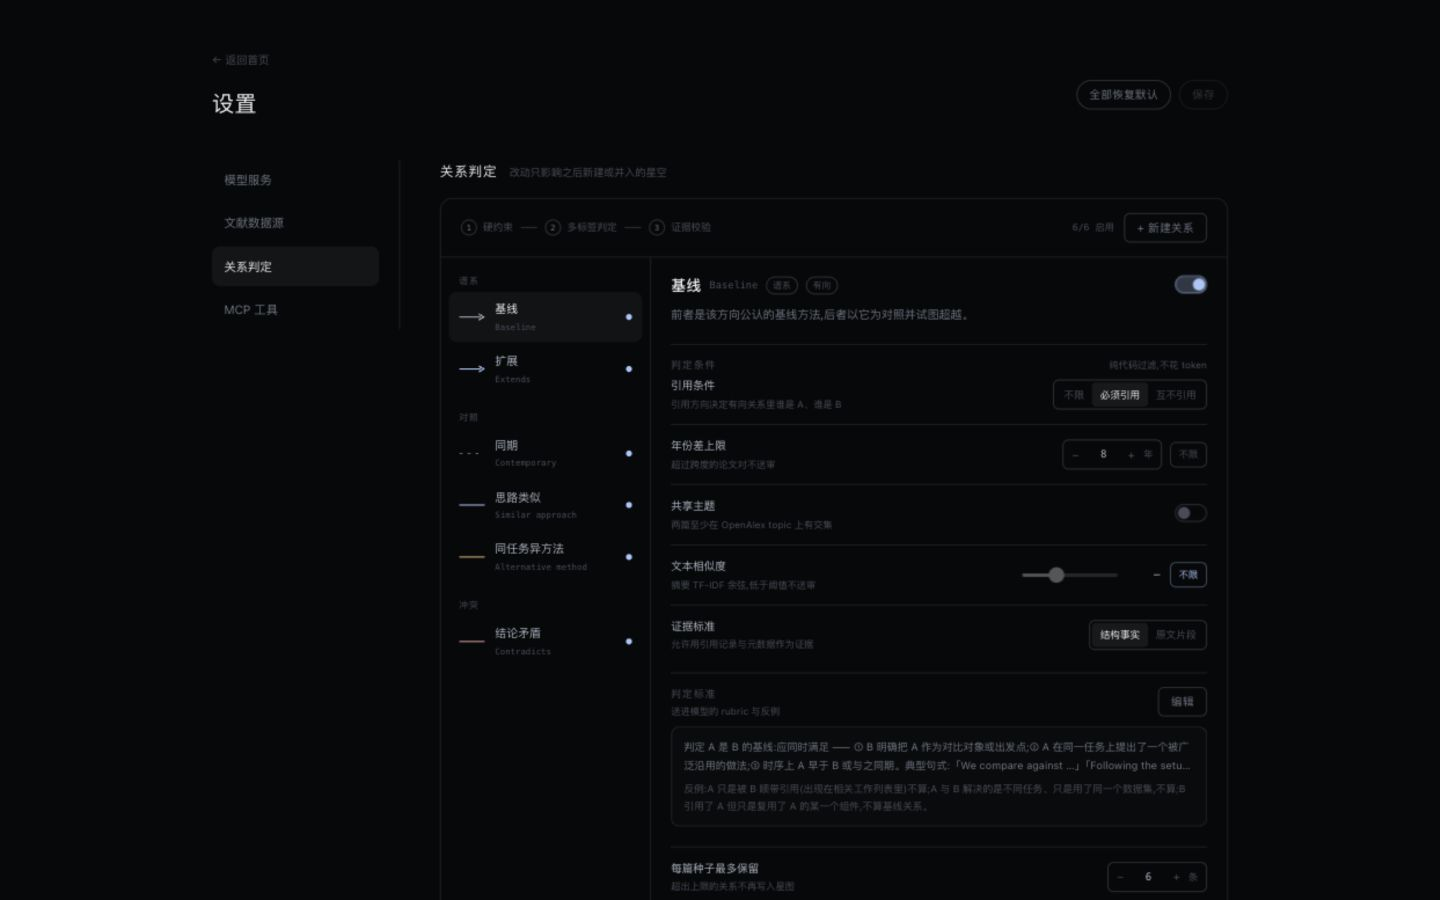
\includegraphics[width=0.84\textwidth]{07-relations.png}
  \caption{关系判定设置：六类关系按用途分组，前置条件、证据标准与反例均可编辑。}
  \label{fig:relations-ui}
\end{figure}

\subsection{证据查看与视觉编码}

图模型里每一种东西在画面上都有唯一对应的表达。论文是一颗星，亮度与被引量相关，半径与年份相关；\code{CITES} 是极细的引力线；基线与扩展是带方向的实线，方向由流动的粒子段表达；同期是虚线，表示“平行但未交汇”；思路类似是冷色实线；同任务异方法是双色调对撞线；结论矛盾是全图唯一的高饱和暖红色；潜在连接是空缺处的暖色细环。\textbf{一色一义}是硬规则：暖红色全图只用于“矛盾”，暖黄色全图只用于“空缺”。颜色一旦复用，视觉编码就失效了。

点开星体，右侧浮窗展示摘要、年份、venue、被引量与该论文的全部关系；点开一条边，展示关系类型、置信度、判定理由与原文证据卡。证据卡里的 \code{span} 片段可以回到对应论文的文本块；引用型证据则显示“谁引用了谁”的上游记录。用户不需要相信一个分数，只需要读一眼原文。

\subsection{文献问答：流式回答、角标与决策轨迹}

问答入口在底部观星台，用户可以输入问题并附最多 4 张图。服务端按“限流 → 预算 → 参数校验 → 输入护栏 → 模型解析 → 检索/规划”的顺序处理，然后创建 SSE 流，把以下事件逐条推给前端：规划步骤、工具调用、检索诊断、证据卡、回答增量、最终引用、决策轨迹与错误。

回答里的 \code{[n]} 角标对应检索到的文本块，点击后定位到星体与原文；图像证据使用 \code{[图1-2]} 这样的独立角标；外部检索结果可以提及，但明确标注“外部检索”，不能伪装成星空内已核验的关系。回答结束后，系统还会从回答里抽取“被提到但星空里还没有”的论文，最多 4 篇，交给用户确认是否加入下一轮种子——这把“问答”与“星空生长”接成了一个闭环。

\begin{figure}[htbp]
  \centering
  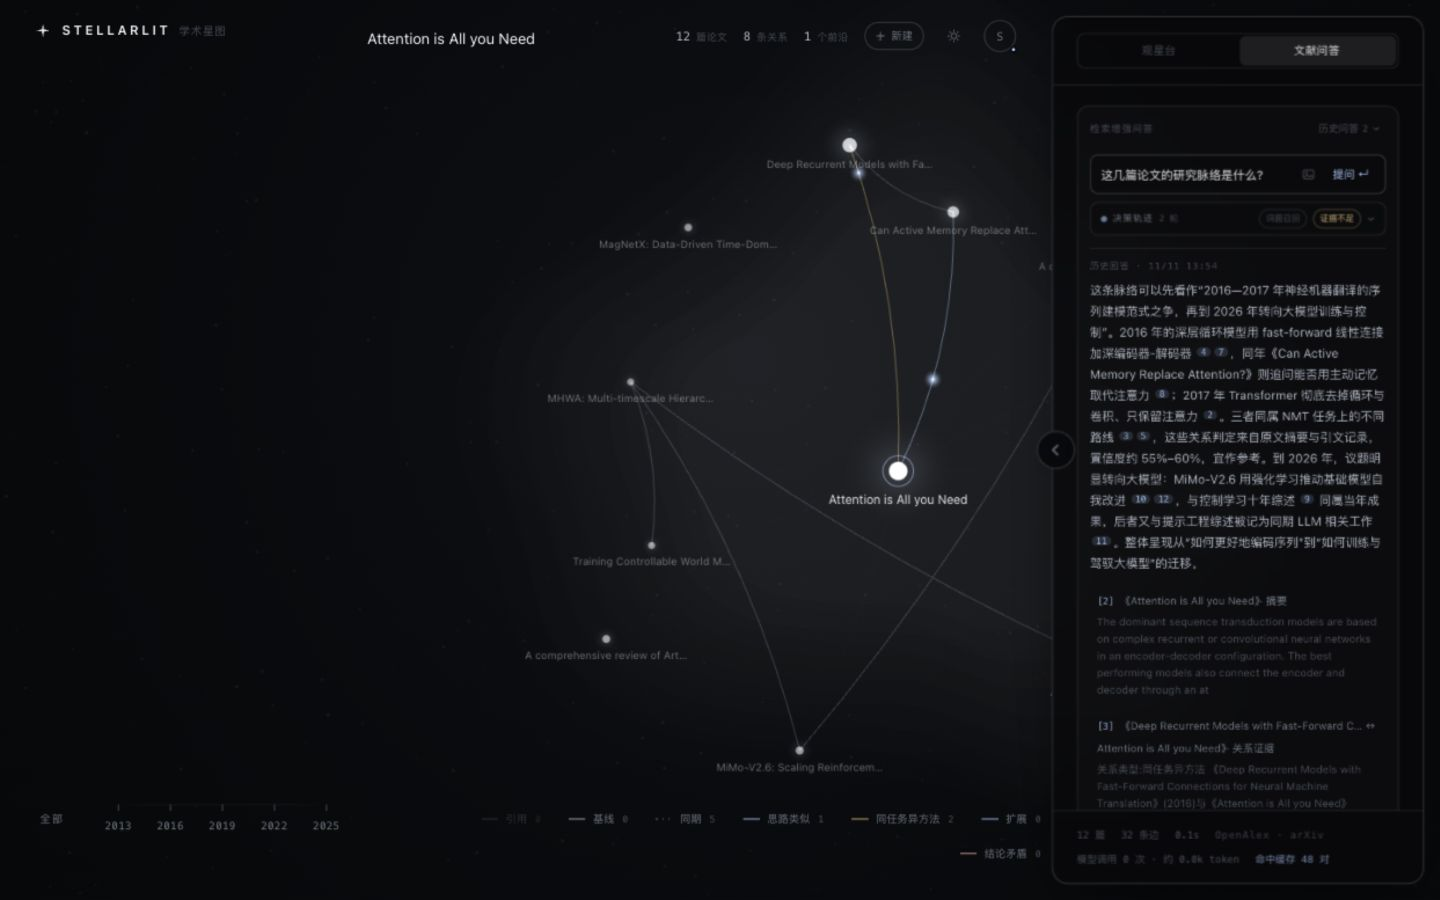
\includegraphics[width=0.84\textwidth]{03-ask.png}
  \caption{文献问答：流式回答、角标引用、检索诊断与 Agent 决策轨迹。}
  \label{fig:ask-ui}
\end{figure}

\subsection{多模态图表问答}

用户上传图表后，视觉模型先做一次结构化抽取，再把结果转成证据块。抽取的内容包括：图像概述、OCR 文字、图表序列、表格行列、关键数值与趋势观察；每个条目可选携带归一化区域坐标。前端把坐标映射到缩略图上的定位框，用户点击角标即可看到“这句话来自图里的哪一块”。

多模态证据与文本证据共享同一套覆盖率与停止判定：如果问题明显在问图（出现“图 / 图表 / 曲线 / 坐标 / 数值 / 趋势”等词），覆盖率门槛会从 0.32 降到 0.22，因为图像块通常只有 OCR、图例与若干数据点，天然比摘要短。图像与正文冲突时，以原图可见内容为准；读不清就明确说不确定，而不是让模型“猜一个合理数值”。

\subsection{MCP：把星空开放给外部 Agent}

MCP 服务把星空能力封装成 9 个只读工具：\code{list_starfields}、\code{get_starfield}、\code{get_paper}、\code{expand_citations}、\code{search_starfield}、\code{find_relation_evidence}、\code{get_paper_context}、\code{resolve_seed}、\code{search_papers}。工具描述是写给模型看的说明书：说清什么时候该用、返回什么、边界在哪；描述写不好，模型就会放着 \code{search_starfield} 不用，退化成瞎猜。

所有工具只读：读存档、查 OpenAlex、检索语料、查两篇之间的已判定关系。改图（并入种子、重跑判定）不在这里——那些要花模型调用和钱，必须由用户确认，不能由一个自己乱逛的 Agent 决定。HTTP 入口使用个人访问令牌：令牌以 \code{slmcp_} 开头，数据库只存 SHA-256，原始令牌只在创建时返回一次；每个账号最多保留 8 个令牌。stdio 入口使用 \code{STELLARLIT_MCP_TOKEN}，与 HTTP 共用同一份工具定义。

\begin{figure}[htbp]
  \centering
  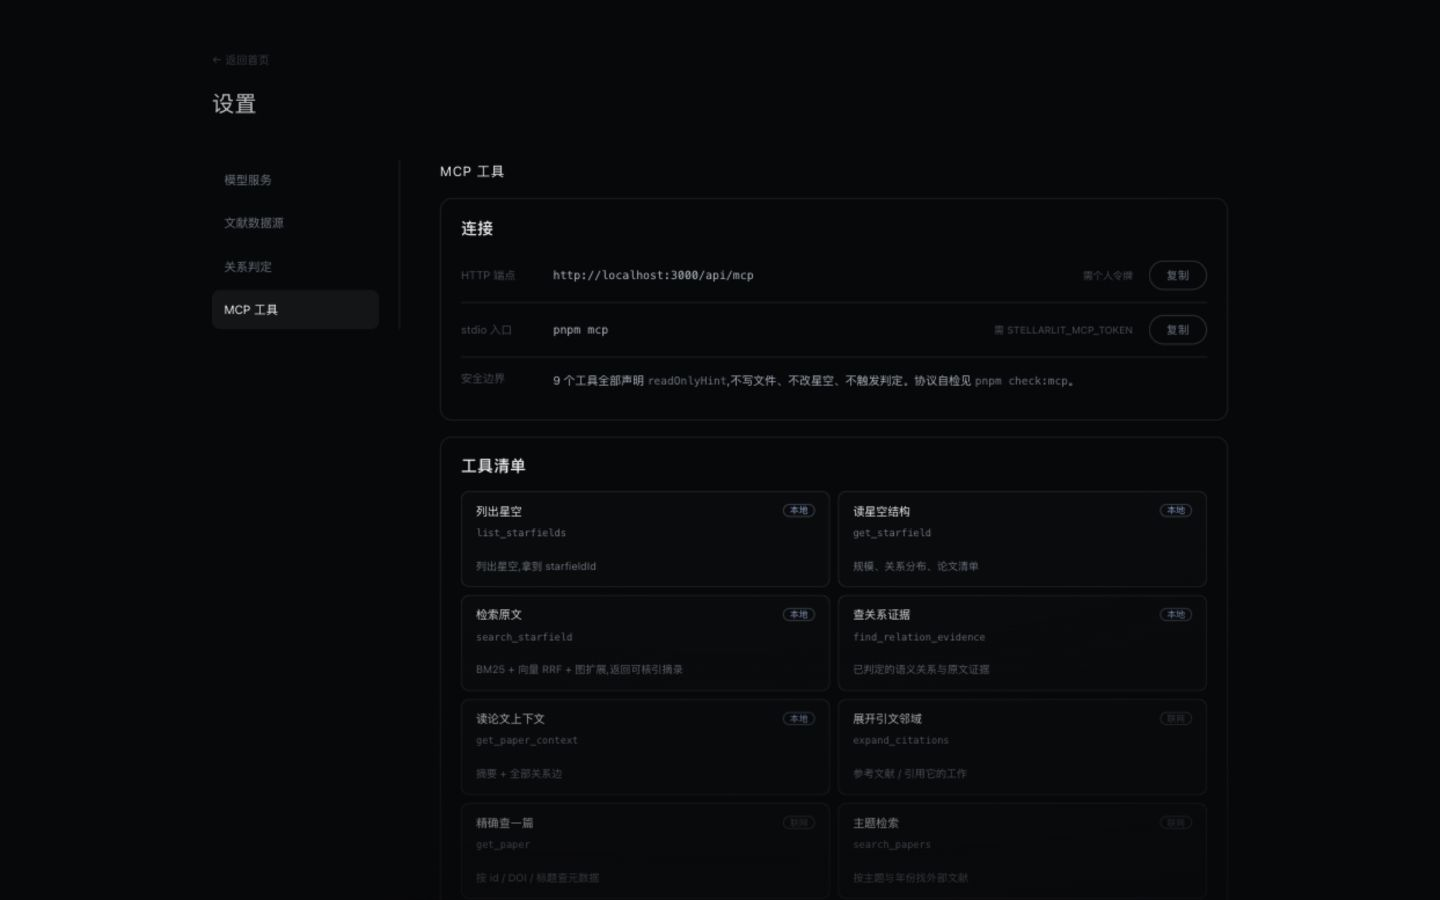
\includegraphics[width=0.84\textwidth]{06-mcp.png}
  \caption{MCP 工具页：只读工具清单、个人令牌与接入配置。}
  \label{fig:mcp-ui}
\end{figure}

\subsection{账号、密钥与用量}

模型服务、向量模型与 Semantic Scholar Key 全部由账号在设置页绑定，系统不读取部署级模型密钥。API Key 使用 AES-256-GCM 加密：12 字节随机 IV、16 字节认证标签、32 字节主密钥，存储格式为 \code{enc:v1:<iv>.<tag>.<ciphertext>}；对外只返回 \code{hasApiKey} 与尾号。主密钥来自 \code{ENCRYPTION_KEY}，丢失后已保存的密钥无法恢复，因此必须与数据库备份分开保管；轮换时把旧密钥放到 \code{ENCRYPTION_KEY_PREVIOUS}，读取仍可用，重新保存一次配置即可全部换成新密钥。

账号隔离有一条容易忽略的迁移规则：首次启动时，旧的演示星空、问答历史、预设与模型配置会被标成 \code{legacy}，由第一个注册的账号自动接管，并在注册响应里说明接管了多少片星空；之后的账号从空开始。MCP 这类机器入口没有 Cookie，用个人令牌绑定 \code{owner_id}；没有令牌或令牌已撤销一律拒绝。

\begin{figure}[htbp]
  \centering
  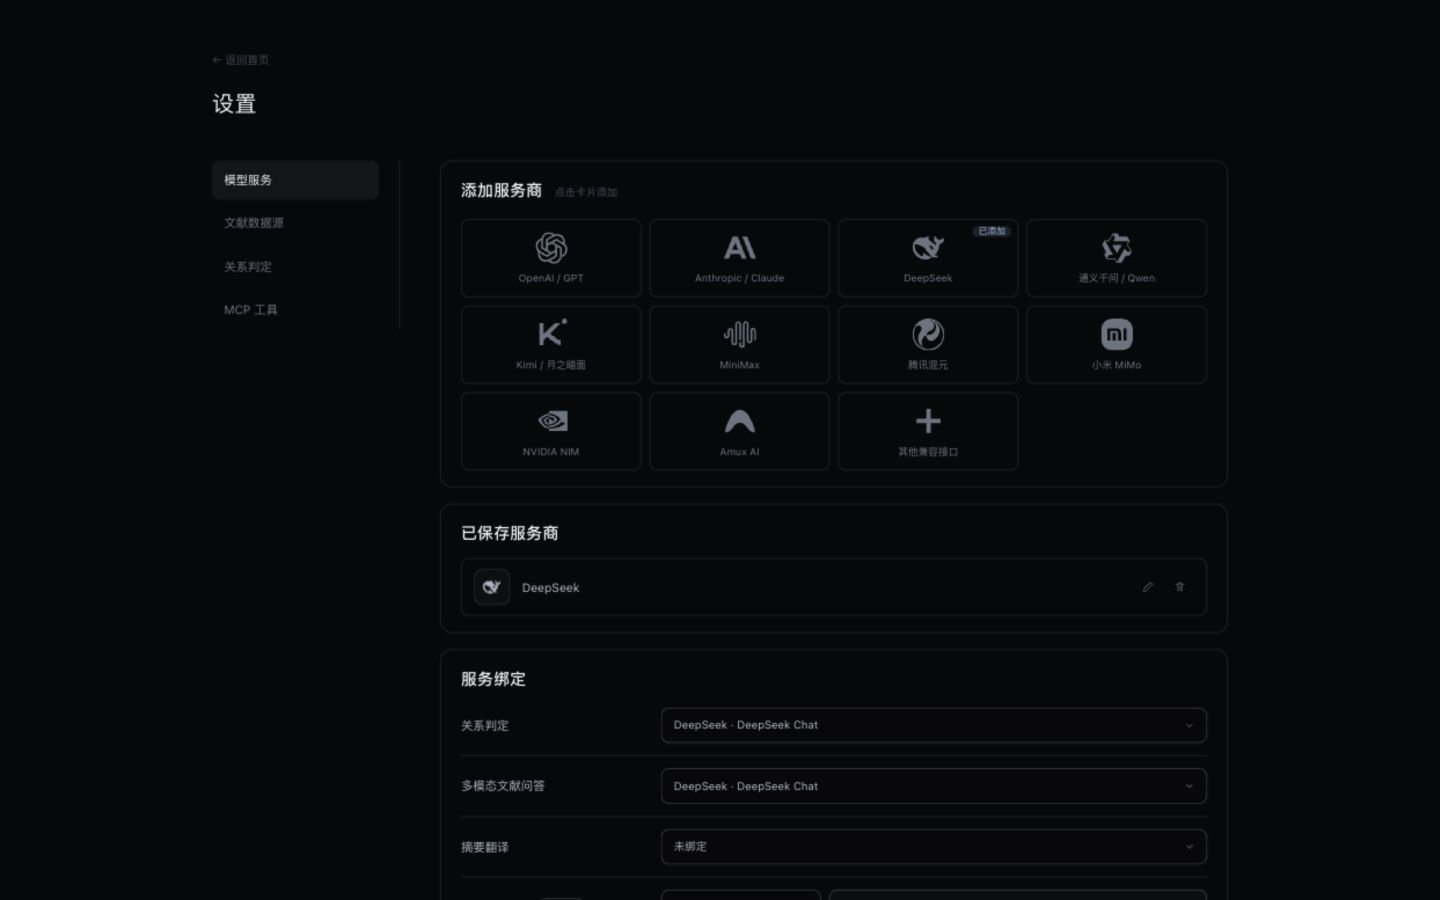
\includegraphics[width=0.84\textwidth]{05-settings.png}
  \caption{模型服务设置：按账号绑定多厂商，分别选择判定 / 问答 / 翻译模型。}
  \label{fig:settings-ui}
\end{figure}

用量按账号累计：每次模型调用按字符数估算 token（中文约 2 字符 1 token，图片每张按 800 token 计），写入 \code{usage} 表；每日预算默认 400000，超出后返回 \code{budget_exhausted} 与剩余额度提示。用量不是为了“卡用户”，而是为了让成本可见：没有度量，优化就无从谈起。
